\chapter{Campo eléctrico atmosférico lento}
\label{ch:background}

%%%%%%%%%%%%% PARTE DE LEO %%%%%%%%%%%%%%%%%%%5
\section{Características de $\vec{E}$ lento}
%README: 
Se define como la componente lenta del campo eléctrico atmosférico, a las variaciones que se dan entre 0.1 Hz a 1 kHz. Una de las principales fuentes de campo eléctrico en la atmósfera se debe a la acumulación de carga en las nubes, sin embargo, la densidad de carga depende del tipo de nube, siendo la nube de tormenta la que posee mayor concentración. Durante su formación los cambios temporales en la carga de la nube producen variaciones lentas del campo eléctrico atmosférico.\\

Cuando la nube está en la etapa inicial del desarrollo, los procesos de generación de carga son la carga por difusión y por deriva o arrastre de carga en el seno de un campo eléctrico (Gunn, 1957) \cite{gunn1957experimental}. A medida que la nube se desarrolla (espesor inferior a 3 Km) comienzan a actuar otros mecanismos como el de selección iónica (captura iónica por gotas polarizadas) (Wilson, 1929; Chalmers, 1967) \cite{stow1969atmospheric } y ruptura (ruptura de gota polarizada por choque) (Matthews and Mason, 1964) \cite{matthews1964electrification}.\\

Por último, cuando la nube está totalmente desarrollada predominan los mecanismos de inducción (transferencia de carga entre gotas polarizadas) (Elster and Geitel, 1913) \cite{elster1913influenztheorie}, convección (captura iónica en corrientes de deriva) (Vonnegut, 1955) \cite{vonnegut1955possible}, termoeléctricos (transferencia de carga entre partículas con diferentes temperaturas) (Latham and Mason, 1961) \cite{latham1961generation} e interfaciales (transferencia de carga a través de la “interface”, por incorporación selectiva de iones, originados por las sales y gases disueltos en el hielo) (Buser and Aufdermaur, 1977) \cite{buser1977electrical}.\\ 

En algunos fenómenos turbulentos de la atmósfera también se puede encontrar variaciones lentas del campo eléctrico. Cuando una nube de tormenta se encuentra totalmente desarrollada, y la carga acumulada es tal que consigue ionizar el medio, se produce una descarga eléctrica atmosférica \cite{garciacampo}, en la Fig. \ref{E_lento} se observa el desarrollo de una descarga atmosférica que inicia con un líder escalonado que crea un camino de baja impedancia por el cual va a transitar la carga y finalmente ocurre la descarga de retorno. Esto se contrasta con el comportamiento del campo eléctrico lento en cada una de las etapas.\\

\begin{figure}[h!]
\begin{center}
\includegraphics[width=1.1\textwidth]{Figures/slow_e_field_graf.png}
\caption[Desarrollo de una descarga eléctrica]{Esquema del desarrollo de una descarga eléctrica, en donde se observa el comportamiento esperado del campo lento en cada una de las fases de la descarga. Primero se da un líder escalonado que crea un camino de baja impedancia por el cual va a transitar la carga y finalmente ocurre la descarga de retorno.}
\label{E_lento}
\end{center}
\end{figure}
Un sistema de campo E lento sería apropiado si se desea estudiar el comportamiento lento (estático) del campo eléctrico atmosférico, el cual se puede dividir en campo eléctrico de buen clima y perturbado, ya que las propiedades son tan diferentes en estos dos tipos de situaciones que, en general, tienden a estudiarse por separado. Esto implica el establecer, a priori, unas condiciones de buen clima. Se considera buen clima cuando no existe precipitación, hay menos de 3/8 de cielo cubierto, y además no existen condiciones extremas de visibilidad o viento \cite{iribarne1980atmospheric}.\\

El campo eléctrico de buen clima es de unos 120 V/m, se dirige hacia el suelo y generalmente presenta una variación diurna, íntimamente ligada a la variación de la resistencia de las capas más bajas de la atmósfera \cite{garciacampo}. El campo eléctrico en condiciones perturbadas se genera por la carga en las nubes y por la concentración de partículas cargadas \cite{hernandez1987pre}.\\


\section{Métodos de detección}
% README: En este apartado se colocará todo lo referente al estado del arte de medición de campo eléctrico lento.
Existen tres mecanismos principales para medir la intensidad del campo eléctrico de CC (Corriente Continua). Estos son las sondas de inducción, molinos de campo y métodos ópticos. Las sondas de inducción miden el potencial de una placa conductora que ha sido equilibrado con el potencial ambiental local con respecto a un plano de tierra de referencia. El molino de campo es similar a la sonda de inducción excepto que la señal de CC se convierte en una señal de CA (Corriente Alterna), ya sea cubriendo y descubriendo alternativamente una placa sensible expuesta a el campo eléctrico local o haciendo oscilar la placa superior de un condensador de placa paralela. En los métodos ópticos el campo eléctrico cambia las propiedades birrefringentes de un cristal sujeto a ese campo, lo que induce un cambio físico en una fibra óptica, alterando así sus propiedades ópticas que luego se analizan \cite{miles2009report}. 
\subsection{Sondas de inducción}
El principio fundamental de una sonda de inducción es permitir que una placa o antena conductora se cargue con el campo local y luego medir el voltaje inducido en la placa como se observa en la Fig. \ref{s1}. Se necesita un circuito de alta impedancia de entrada para poder medir la carga inducida en la placa. Se usa el plato de inducción como una de las placas del capacitor y la superficie sensible cargada como la otra, tal como se observa en la Fig. \ref{s2}  \cite{miles2009report}. En los capacitores de placas paralelas, la carga inducida se relaciona con la diferencia de potencial entre sus placas por medio de la Eq. \ref{eqq1}.
\begin{equation}
    C = \frac{Q}{V_{Plato\, de\, inducci\acute{o}n} - V_{Superficie\, sensible}}
    \label{eqq1}
\end{equation}
La capacitancia C es conocida y esta dada por la Eq \ref{eqq2}, donde $\epsilon$ es la permitividad del aire, A es el área de los platos y d es la separación de las placas. La sonda se calibra con campos eléctricos inducidos controlados.
\begin{equation}
    C =  \frac{\epsilon A}{d}
    \label{eqq2}
\end{equation}
Uno de los principales problemas de este sensor, es que no posee un sistema natural de descarga, por lo que se utilizan métodos electrónicos y mecánicos para descargar la superficie sensible.\\

\begin{figure}[h!]
 \centering
  \subfloat[]{
   \label{s1}
    \includegraphics[width=0.4\textwidth]{Figures/sonda_a.eps}}
  \subfloat[]{
   \label{s2}
    \includegraphics[width=0.5\textwidth]{Figures/sonda_b.eps}}
 \caption[Sonda de inducción de campo eléctrico]{(a) En este esquema se muestra el plato en el que se induce carga por el efecto capacitivo, seguido del circuito de alta impedancia utilizado para medir las variaciones de carga, (b) Capacitor de placas paralelas utilizado para medir las variaciones de campo eléctrico, la carga que se induce en la superficie sensible se replica en el plato de inducción y esta es medida por el circuito de alta impedancia. }
 \label{sonda}
\end{figure}

\subsection{Molino de placas}
Una técnica común para medir campos eléctricos de CC es mediante un obturador que gira sobre un condensador de medición generando una señal oscilante. En la Fig. \ref{mill} se muestra un esquema básico de un molino de campo. La conversión de la medición del campo eléctrico de un campo de CC a una señal de CA ayuda a minimizar los efectos de las interferencias espurias, las deriva y los efectos de carga espacial. Los molinos de campo son más complejos y por lo tanto más costosos que los sistemas de placa de inducción, pero exhiben mayor sensibilidad sin necesidad de implementar un sistema electrónico que permita descargar las placas sensibles. El campo eléctrico se obtiene de la Eq. \ref{corr1}, 
\begin{equation}
    I = \epsilon E \frac{dA}{dt}
    \label{corr1}
\end{equation}
donde $\epsilon$ es la permitividad del aire, $E$ es el campo eléctrico inducido y A es el área sensible que depende del tiempo de exposición.\\

\begin{figure}[h!]
\begin{center}
 \includegraphics[width=0.6\textwidth]{Figures/emill.png}
\caption[Esquema básico del sensor de campo tipo molino]{Esquema básico de un molino de campo eléctrico, donde se observa el campo incidente $\overrightarrow{E}$, que es filtrado por la placa superior que gira a un velocidad $W_{s}$, el plato sensible se carga y descarga en relación al giro de la placa.}
\label{mill}
\end{center}
\end{figure}

\subsection{Molino cilíndrico}

Un segundo tipo de molino de campo es el molino cilíndrico el cual se muestra en la Fig. \ref{schema}. Este molino gira sobre el eje perpendicular al campo impuesto. La corriente de CA resultante está relacionada con el campo eléctrico a través de la Eq. \ref{cilind},
\begin{equation}
    I = 4 \epsilon_{0} r L E \cos(\omega t)
    \label{cilind}
\end{equation}
donde $r$ es ahora el radio del cilindro y $L$ es la longitud del cilindro que gira perpendicularmente al campo $E$, a una frecuencia angular $\omega$. Los dispositivos cilíndricos tienen la ventaja de ser insensibles a pequeñas fugas de carga y puede medir campos con precisión. Estas sondas son direccionales y no pueden detectar campos paralelos a su eje midiendo de esta manera la orientación del campo.\\

JPL(Jet Propulsion Laboratory) ha utilizado sensores cilíndricos de campo eléctrico para estudios atmosféricos \cite{johnston1989miniaturized}, pero no hay vendedores comerciales conocidos para estos dispositivos. La versión actual tiene un rango de 0.05 kV/m hasta 100 kV/m \cite{johnston1989miniaturized}.\\

\begin{figure}[h!]
\begin{center}
\includegraphics[width=0.6\textwidth]{Figures/Cilindrico_mill.PNG}
\caption[Esquema básico del sensor tipo molino cilíndrico]{Esquema básico del sensor de molino cilíndrico, donde se puede observar el mecanismo de inducción de carga que posee \cite{renno2008miniature}.}
\label{schema}
\end{center}
\end{figure}
\subsection{Micro-sensor de campo eléctrico}
El micro-sensor mecánico es muy pequeño en comparación al convencional molino de campo, convencionalmente se fabrican de 10 mm$^{2}$ de área. Posee una serie de laminas de 1 mm$^{2}$ que vibran gracias a actuadores térmicos, eliminando así el desgaste asociado con la rotación y el movimiento de los electrodos del molino de campo. El sensor requiere una potencia de funcionamiento mínima de 70 $\mu$W. El micro-sensor de campo funciona a 4200 Hz, lo cual permite la medición de campo eléctricos rápidos (1 kHz a 1 MHz) y lento (0.1 Hz a 1 kHz). Dos juegos de electrodos habilitan la medición diferencial y, por lo tanto, no requiere un potencial de tierra de referencia \cite{wijeweera2009micromachined}.\\

El sensor tiene una respuesta lineal a la amplitud del campo y ha demostrado ser capaz de medir un campo de CC tan pequeño como 42 V/m. En la Fig. \ref{micromachine} se observa el esquema eléctrico del sensor y una imagen del prototipo construido por el departamento de ingeniería eléctrica e informática, de la Universidad de Manitoba, Canadá.\\

\begin{figure}[h!]
\begin{center}
\includegraphics[width=0.7\textwidth]{Figures/microsensor.PNG}
\caption[Micro sensor de campo eléctrico]{Prototipo de micro sensor de campo eléctrico, el cual utiliza actuadores térmicos para hacer vibrar un conjunto de laminas que cubren y descubren placas sensibles que captan el campo eléctrico \cite{wijeweera2009micromachined}.}
\label{micromachine}
\end{center}
\end{figure}
\subsection{Sensores Ópticos}
Una desventaja de los métodos de medición descritos anteriormente es que la presencia misma de los sensores metálicos perturba el campo eléctrico. Los sensores ópticos no afectan el campo que se mide. Estos sensores generalmente se basan en el efecto de Pockel’s donde un campo eléctrico cambia las propiedades birrefringentes de un cristal sujeto a ese campo y el cambio resultante en la polarización de la luz láser que atraviesa el cristal es medido utilizando una variedad de arquitecturas de sistemas ópticos. Este tipo de sensores miden campos eléctricos de CC hasta unos 10 kV/m con resoluciones de 100 V/m \cite{miles2009report}. En la Fig. \ref{optical} se muestra el esquema de un sensor de campo óptico, compuesta principalmente por la antena, la fibra óptica y la unidad sensora.\\

\begin{figure}[h!]
\begin{center}
\includegraphics[width=.8\textwidth]{Figures/optical_sensor.PNG}
\caption[Esquema del sensor optico de campo eléctrico]{Esquema general del sensor óptico compuesto principalmente por la antena, la fibra óptica y la unidad sensora \cite{miles2009report}.}
\label{optical}
\end{center}
\end{figure}
\section{Diseño del sensor de $\vec{E}$ lento}
Teniendo en cuenta sus propiedades de medición y su bajo costo se optó por construir un sensor de campo tipo molino. Las placa sensible de área $A$ es expuesta a un campo eléctrico uniforme durante un tiempo $T$ con cada giro del obturador, tal como se observa en la Fig. \ref{mill}.\\

La ley de Gauss establece que el flujo eléctrico de una superficie cerrada es igual a la carga encerrada dividida por la permitividad $\epsilon_{0}$, es decir,
\begin{equation}
    \phi = \oint \vec{E}.dA= \frac{q}{\epsilon_{0}}
\label{Eq1}
\end{equation}
Con la ecuación \ref{Eq1}, la carga $q$ inducida en la placa sensible se puede expresar como,
\begin{equation}
    q = \epsilon_{0} E A
\label{Eq2}
\end{equation}
El campo eléctrico puede ser directamente determinado por la medición de la carga inducida, que es proporcional al campo incidente. El medidor de campo de aspas giratorias, que se muestra en la Fig. \ref{emill1}, utiliza un rotor conectado a tierra que cubre y descubre periódicamente la superficie $A$ del sensor del campo eléctrico. El número de aspas del molino define la cantidad de veces que el sensor estará expuesto al campo eléctrico durante cada rotación del motor. Por lo tanto, la superficie del sensor A(t) en la que se induce la carga q(t) varia linealmente con el tiempo, y se define como,
\begin{equation}
    \frac{dq(t)}{dt} = i(t) = \epsilon_{0} E \frac{dA(t)}{dt}
\label{Eq3}
\end{equation}
La variación $\frac{dA(t)}{dt}$, que representa al área expuesta al campo en función del tiempo, depende de la velocidad angular del motor y de la cantidad de aspas del molino \cite{tant2007design}.

\begin{figure}[h!]
\begin{center}
\includegraphics[width=.55\textwidth]{Figures/Emill.eps}
\caption[Esquema del sensor tipo molino fabricado]{Esquema del sensor de molino de campo eléctrico, donde se nombra cada una de de sus componentes, el sensor esta compuesto principalmente por la placa sensible, la placa del molino, el dieléctrico,la placa de tierra, un motor y un encoder que mide la fase de giro.}
\label{emill1}
\end{center}
\end{figure}

El diseño que se propuso se muestra en la Fig. \ref{emill1}, a diferencia de los modelos comerciales, este posee una placa dieléctrica de acrílico, que aumenta la capacitancia y por ende, la carga que pueden almacenar las placas, en la Fig. \ref{emill_c} se encuentra el esquema completo del sensor donde se muestra cada una de las etapas por las que atraviesa la señal medida.\\

\begin{figure}[h!]
\begin{center}
\includegraphics[width=1\textwidth]{Figures/Emill_esquema.eps}
\caption[Esquema de las etapas del sensor de campo eléctrico tipo molino]{Esquema completo del sensor, compuesto por la electrónica de acondicionamiento, adquisición y transmisión datos.}
\label{emill_c}
\end{center}
\end{figure}

La señal de salida de la placa sensora es de naturaleza senoidal, esto debido a la carga y descarga que causa el obturador al pasar sobre los platos. La acumulación de carga en las placas, produce una corriente, que es medida utilizando un conversor corriente a tensión, seguido de un sistema de acondicionamiento que permite la rectificación de la señal utilizando un rectificador de precisión. Finalmente, se utiliza un filtro pasa bajas pasivo para extraer la componente DC de la señal la cual es digitalizada y transmitida mediante el protocolo I$^{2}$C.
\subsection{Fabricación del sensor tipo molino}

Para el diseño de un sensor de molino de campo eléctrico, es necesario seleccionar cuidadosamente los parámetros de fabricación, ya que estos afectan directamente la medición. Los parámetros a tener en cuenta son el área, la cantidad de aletas, velocidad de giro del motor y material de las placas.\\

En la construcción del sensor se utilizó 3 placas de baquela de 1.4 mm de espesor y un recubrimiento de cobre de 35 $\mu$m y para la placa dieléctrica se utilizó una lamina de acrílico de 2 mm de espesor. Entre las placas de cobre encontramos la placa sensible de 62 mm de diámetro que esta compuesta por 3 aspas separadas 60$^{\circ}$ entre sí (ver Fig. \ref{real1}), el obturador posee la misma geometría del plato sensible y una pestaña de 5 mm en cada aspa para medir la fase de giro con un enconder (ver Fig. \ref{schema1}), la placa de referencia a tierra es circular de 62 mm de diámetro y posee un orificio de 4 mm en su centro por donde pasa el eje del motor. La placa dieléctrica de acrílico es circular de 62 mm de diámetro y 2 mm de espesor, también posee un orificio de 4 mm para el eje del motor.\\

\begin{figure}[h!]
 \centering
  \subfloat[]{
   \label{schema1}
    \includegraphics[width=0.4\textwidth]{Figures/obturador.png}}
  \subfloat[]{
   \label{real1}
    \includegraphics[width=0.4\textwidth]{Figures/sensor.png}}
 \caption[Esquema de las placas del sensor de campo tipo molino]{(a) Obturador de cobre de 3 aspas con separación de 60$^{\circ}$ entre aspa, el radio es de 36 mm, 5 mm más que la placa sensora, para poder medir la fase de giro con un elemento opto-detector, el obturador posee un orificio central de 2 mm para el eje del motor, (b) Placa sensora de cobre, de radio 31 mm, el orificio central es 2 veces más grande en comparación al obturador (4 mm), para evitar que el eje de giro entre en contacto con la placa sensible.}
 \label{placas}
\end{figure}
El acrílico posee típicamente una permitividad dieléctrica relativa $ k = 4$, ya que la carga almacenada es proporcional a la capacitancia \cite{westerlund1994capacitor}, añadir un pieza de acrílico tiene el efecto ideal de aumentar un factor de 4 la cantidad de carga almacenada en el capacitor conformado por la placa sensible y la placa de referencia a tierra, en la Eq. \ref{capac} se puede observar la relación entre la carga almacenada y la permitividad dieléctrica del material,
\begin{equation}
    Q=kC_{0}V_{0}
    \label{capac}
\end{equation}
\begin{equation}
    C_{0}=\frac{\epsilon_{0}A}{d}
    \label{capc2}
\end{equation}
donde $Q$ es la carga almacenada, $k$ es la permitividad relativa del material, C$_{0}$ es la capacitancia de las placas en el vacío, V$_{0}$ es el voltaje de las placas, A es el área de las placas,d la separación entre ellas y finalmente $\epsilon_{0}$ es la constante de permitividad del vacío. Con la Eq. \ref{capc2} es posible estimar el valor de capacitancia del sensor, inicialmente se calcula el área de la placa sensible, la cual viene dada por la Eq. \ref{area},
\begin{equation}
    A = \frac{\pi }{2}\left [ 3R^{2}-r^{2} \right ]
    \label{area}
\end{equation}
el área estimada de la placa sensible es de 4,34 mm$^{2}$ y la distancia de separación $d$ es de 3 mm, donde 1 mm corresponde al aire y 2 mm al dieléctrico, la capacitancia total es de 24,45 $\rho$F, para el caso en el que no se adiciona un dieléctrico, la capacitancia es de 12.81 $\rho$F. Como se presento en la Eq. \ref{capac}, un aumento en la capacitancia implica un mayor almacenamiento de carga, y por tanto un aumento en la amplitud de la señal censada, de esta forma se mejora el rango de medición.\\

A la hora de seleccionar el material de las placas, se encontró que los materiales usualmente utilizados son el cobre y el aluminio, por lo que se realizaron pruebas de laboratorio en donde se comparó dos sensores de cada material con una frecuencia de giro de 87 Hz expuestos a un campo eléctrico constante de 16 kV/m.
\begin{figure}[h!]
\begin{center}
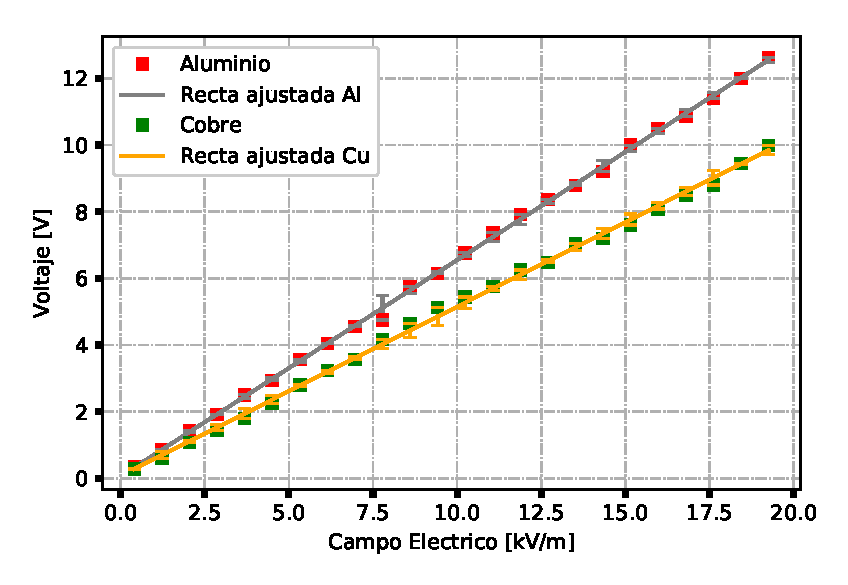
\includegraphics[width=0.8\textwidth]{Figures/Al_vs_Cu.eps}
\caption[Gráfica del voltaje inducido para distintos materiales]{Gráfica del voltaje inducido en un sensor emill con electrodo de cobre (verde) y un sensor emill con electrodo de aluminio (rojo). Ambos electrodos de 62 mm de diámetro, el motor girando a 87 Hz y un campo eléctrico constante incidente de 16 kV/m.}
\label{alcu}
\end{center}
\end{figure}
Los resultados se encuentran en la Fig. \ref{alcu}, en donde se observa que el aluminio posee mejor respuesta, sin embargo considerando la complejidad que conlleva trabajar con este material y haciendo notar que la diferencia en las respuestas es menor al 20\%, se opta por trabajar con cobre.\\

Para seleccionar la velocidad de giro óptima se realizaron pruebas de laboratorio variando la velocidad del motor y observando el voltaje inducido en las placas del sensor, los resultados de las pruebas arrojaron los resultados que se observan en la Fig. \ref{fv}.
\begin{figure}[h!]
\begin{center}
\includegraphics[width=0.8\textwidth]{Figures/Frec_vs_Vind.eps}
\caption{Gráfica del voltaje inducido vs la frecuencia de giro del motor para un campo eléctrico constante de 16 kV/m.}
\label{fv}
\end{center}
\end{figure}
Ya que el motor tenía un límite de 9 V en la alimentación definido por el fabricante, se estableció un rango de frecuencias de 100 Hz a 600 Hz. Para seleccionar la velocidad adecuada para el motor se tuvieron en cuenta el consumo de energía, la vibración y el ruido auditivo,  por lo que se decidió trabajar con un frecuencia de giro de 87 Hz, obteniéndose una señal sinusoidal de 260 Hz aproximadamente.

\subsection{Conversión corriente a tensión}
El movimiento del obturador permite la carga y descarga de la placa sensible, y en consecuencia, el área efectiva de la placa en la que se inducen cargas debido al campo eléctrico varía con el tiempo. Esta variación temporal de área genera una corriente eléctrica que fluye desde la placa sensitiva, tal como se observó en la Eq. \ref{Eq3}.\\

Debido a que la corriente que fluye desde la placa sensitiva es del orden de micro-amperios, es necesario implementar una topología que nos permita medirla, el circuito se muestra en la Fig. \ref{iv}. El circuito esta compuesto por un seguidor de voltaje tipo buffer y un divisor de tensión resistivo, los valores de resistencia se escogieron teniendo en cuenta el rango de medición del sensor. El voltaje en la resistencia R2 se mide con un seguidor de voltaje para acoplar impedancias entre el divisor y el circuito posterior de acondicionamiento.\\

\begin{figure}[h!]
\begin{center}
\includegraphics[width=.5\textwidth]{Figures/I-V.eps}
\caption{Circuito conversión corriente a tensión.}
\label{iv}
\end{center}
\end{figure}
El rango de medición del sensor se escogió teniendo en cuenta el valor de campo eléctrico mínimo que logra desencadenar un RREA (por sus siglas en inglés Relativistic Runaway Electron Avalanche), siendo este de aproximadamente 286 kV/m\cite{skeltved2017constraints}. La relación de ganancia del divisor de voltaje viene dado por la Eq. \ref{rel}, siendo R1 de 1 M$\Omega$ y R2 un potenciómetro de 500K que se establece en aproximadamente 80 k$\Omega$ con lo cual se consigue una relación de voltaje entrada-salida de aproximadamente $\frac{1}{15}$.
\begin{equation}
    \frac{Vin}{Vout}=\frac{R1}{R1+R2}=\frac{1}{15}
    \label{rel}
\end{equation}
Para simular el circuito \ref{iv}, se utilizó el programa LTspice de licencia abierta, la carga entregada por la placa sensora se recreó con una fuente de corriente, se estableció la relación de ganancia tal como se muestra en la Eq. \ref{rel}, los resultados se observan en la Fig. \ref{ivgraf}, en la gráfica se tienen dos ondas de diferente color, la onda naranja representa la señal de corriente que es del orden de micro-amperios, y la onda azul representa el voltaje a la salida de la etapa buffer.\\

\begin{figure}[h!]
\begin{center}
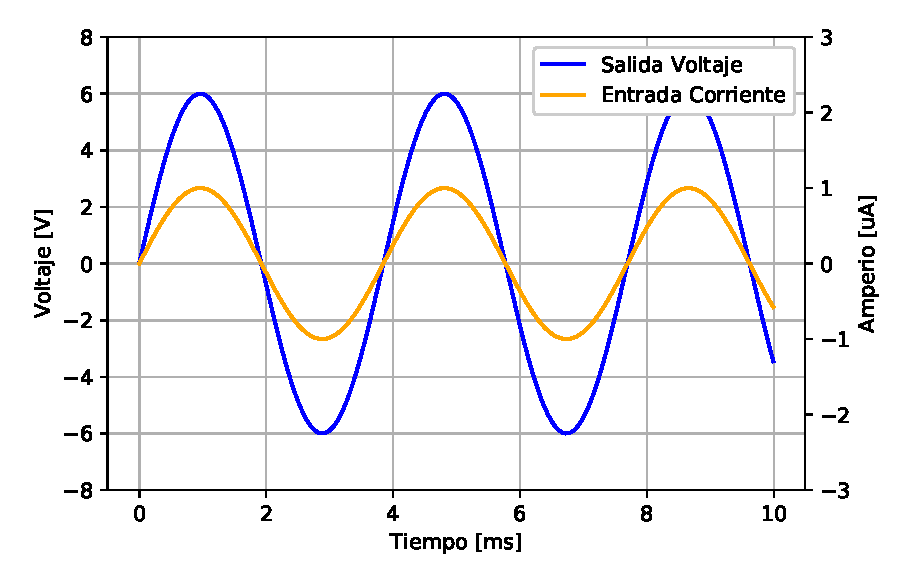
\includegraphics[width=0.8\textwidth]{Figures/I_V_graf.eps}
\caption[Gráfica de la simulación de la etapa corriente a tensión]{Gráfica obtenida de la simulación en LTspice del circuito \ref{iv}, la linea naranja representa la corriente que entrega la placa sensible, la azul es la onda de voltaje que se obtiene del divisor de resistivo, la atenuación del divisor resistivo aumenta el rango de medición en un factor de 15.}
\label{ivgraf}
\end{center}
\end{figure}

\subsection{Acondicionamiento de la señal}

Una de las propiedades más importantes del sensor de tipo molino, es que permite determinar la dirección del campo eléctrico vertical comparando la fase de giro del obturador y la fase de la señal que se induce en el plato sensible, para realizar esta comparación se utiliza el sistema embebido PSOC 5LP. Un PSOC (Programmable System on Chip) es un dispositivo fabricado por la empresa Cypress, esta conformado por microcontroladores cuya principal característica es contar con módulos tanto análogos como digitales en un solo chip, así mismo poder reconfigurar dinámicamente las entradas y salidas de estos módulos.\\

Para este proyecto se utilizó la tarjeta PSOC 5LP (ver Fig. \ref{psoc}), que cuenta con su propio kit de programación, procesador CPU ARM Cortex-M3, coprocesador DFB de hardware de 24 bits, opamps, PGA, filtros, comparadores, ADC SAR y Delta-Sigma y detección táctil CapSense. Las entradas analógicas del PSOC 5LP, manejan rangos de voltajes que van desde 0 V a 5 V, y la señal que se obtiene de la etapa de conversión corriente a tensión varia entre -12 V y 12 V, es por esto que se implemento un circuito de acondicionamiento (ver Fig. \ref{rs}), que reduce la amplitud y suma un nivel de DC a la señal de tal manera que se aproveche el rango de medición.\\

\begin{figure}[h!]
\begin{center}
\includegraphics[width=.8\textwidth]{Figures/psoc.png}
\caption[Kit programable PSOC 5LP]{Kit programable PSOC 5LP, conformado por microcontroladores cuya principal característica es contar  con módulos tanto análogos como digitales en un solo chip.}
\label{psoc}
\end{center}
\end{figure}

\begin{figure}[H]
\begin{center}
\includegraphics[width=.8\textwidth]{Figures/red_sum.eps}
\caption[Etapa de acondicionamiento de la señal]{Etapa de-amplificadora inversora de ganancia $1/5$, seguida de un restador de ganancia unitaria, que revierte la fase y le suma un nivel de offset.}
\label{rs}
\end{center}
\end{figure}

La etapa amplificadora inversora, relaciona el voltaje de entrada y salida por medio de la Eq. \ref{ganrs}, por lo que si se estable R4$>$R5, se puede de-amplificar la señal de entrada. Se escogió $R4=33\,k\Omega$ y $R5=6.8\,k\Omega$ para aprovechar el rango completo de los pines analógicos del PSOC, la ganancia que se obtiene es de $G=-\frac{1}{5}$, y en consecuencia, la señal a la entrada de la etapa se reduce a un rango entre -2.5 V y 2.5 V.
\begin{equation}
    V_{out}=-\frac{R_{5}}{R_{4}}V_{in}
    \label{ganrs}
\end{equation}
La etapa amplificadora inversora redujo la amplitud de la señal e invirtió la fase, por lo que en la siguiente etapa es necesario sumar un nivel de DC para cubrir el rango de medición de los pines analógicos e invertir nuevamente la fase de la señal, esto se logró mediante una etapa amplificadora restadora.
\begin{equation}
    Vout = \frac{R_{2}}{R_{1}}\left (V_{2}-V_{1} \right )
    \label{gres}
\end{equation}
En la Fig. \ref{rs}, se observa la topología y los valores de resistencias que se utilizaron para la etapa amplificadora restadora. Si $R6=R9$ y $R7=R8$ la relación entre la entrada y salida viene dada por la Eq. \ref{gres}, donde V1 es la señal que va a la entrada inversora y V2 a la entrada no inversora, el nivel de DC se escogió experimentalmente midiendo valores de campo eléctrico, se encontró que 2.225 V es el valor para el cual el campo eléctrico se aproxima a 0 V/m. En la Fig. \ref{rsgraf} encontramos los resultados de la simulación en LTspice del circuito de la Fig. \ref{rs}, donde la linea azul representa la señal que entrega la etapa de conversión corriente a tensión, y en naranja la señal después de aplicar la etapa de acondicionamiento, que redujo 5 veces la señal de entrada y sumo un nivel de DC de 2.225 V. 

\begin{figure}[H]
\begin{center}
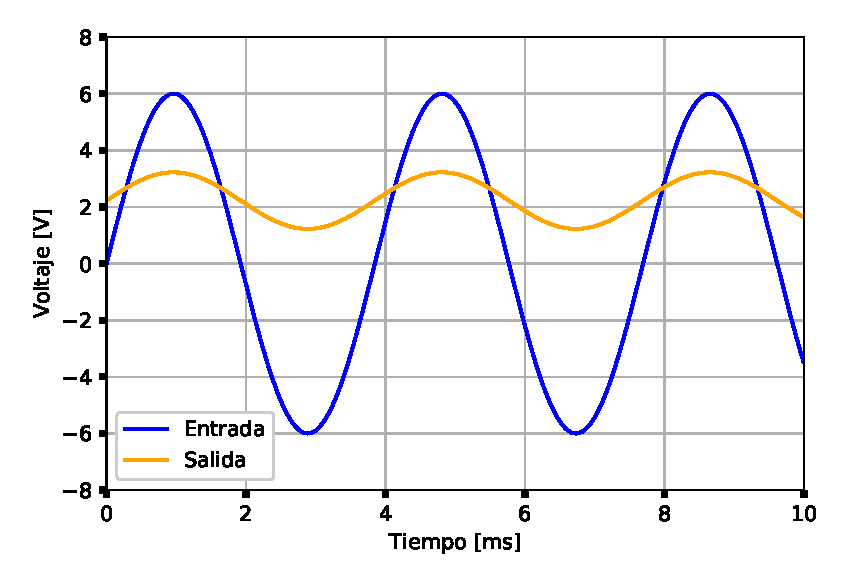
\includegraphics[width=.8\textwidth]{Figures/red_sum_graf.eps}
\caption[Simulación de la etapa de acondicionamiento de la señal]{Gráfica obtenidas de la simulación en LTspice del circuito  de la Fig. \ref{rs}, donde la linea azul representa la señal que entrega la etapa de conversión corriente a tensión, y en naranja la señal después de aplicar la etapa de acondicionamiento, que redujo 5 veces la señal de entrada y sumó un nivel de DC de 2.225 V}
\label{rsgraf}
\end{center}
\end{figure}
Los resultados de la implementación de la etapa de acondicionamiento se muestran en la Fig. \ref{acondicionamiento}, donde se observa la señal inducida en el sensor (azul), que corresponde a un campo eléctrico de 50 kV/m y la señal que se obtiene a la salida de la etapa de acondicionamiento (amarilla), la cual posee un nivel de DC de 2.35 V y se a reducido en un factor de $\sim$6.\\

\begin{figure}[H]
\begin{center}
\includegraphics[width=.8\textwidth]{Figures/Adec_signal.PNG}
\caption[Mediciones realizadas a la salida y entrada de la etapa de acondicionamiento]{Resultados de la implementación de la etapa de acondicionamiento, donde se observa la señal inducida en el sensor (azul), que corresponde a un campo eléctrico de 50 kV/m y la señal que se obtiene a la salida de la etapa de acondicionamiento (amarilla), la cual posee un nivel de DC de 2.35 V y se a reducido en un factor de $\sim$6.}
\label{acondicionamiento}
\end{center}
\end{figure}
\subsection{Etapa rectificadora de precisión}
% README: Explicación de la etapa, esquema del circuito, PSOC, primeras mediciones.
Con el fin de obtener una señal de DC que sea proporcional a las variaciones de campo eléctrico atmosférico, se implementó una etapa rectificadora de precisión utilizando el sistema embebido PSOC 5LP, el cual cuenta con el módulo MIXER (ver Fig. \ref{modulo}) que permite aplicar la operación de rectificación tomando como parámetros la señal que se obtiene de la etapa de acondicionamiento, la señal de la fase de giro del obturador la cual es medida con un encoder (EE-SJ3) y un voltaje de referencia que le indica al módulo en que nivel de offset aplicar la operación.\\

\begin{figure}[h!]
 \centering
  \subfloat[]{
   \label{modulo}
    \includegraphics[width=0.35\textwidth]{Figures/rect.eps}}
  \subfloat[]{
   \label{config_modulo}
    \includegraphics[width=0.65\textwidth]{Figures/mixer_config.PNG}}
 \caption[Módulo MIXER PSOC 5LP]{(a) Esquema del módulo MIXER, el cual tiene como entradas, la señal que entrega la etapa de acondicionamiento, la fase de giro del obturador medida con un encoder y un nivel de DC que establece el voltaje de operación del módulo. (b) Configuración del módulo hecha en el software de desarrollo PSOC Creator.}
 \label{mixer}
\end{figure}
El módulo MIXER hace parte de un conjunto amplio de librerías que se encuentra disponibles en el software PSOC Creator en su versión 4.2 libre de la empresa Cypress. En la Fig. \ref{config_modulo} se observa la configuración del módulo, se estableció la frecuencia de entrada de la señal en 300 Hz debido a que el módulo opera sobre un rango de frecuencia que va desde 0 Hz hasta el valor de frecuencia que se establece en el parámetro, también se escogió reloj externo ya que de esta forma podemos definir la señal que se obtiene del encoder que corresponde al la fase de giro del obturador como el reloj del módulo.

\begin{figure}[h!]
\begin{center}
\includegraphics[width=.8\textwidth]{Figures/rect_pos.eps}
\caption[Operación del módulo MIXER, con una señal en fase al giro del motor]{Gráfica de la operación del módulo MIXER, la señal azul representa la salida de la etapa de acondicionamiento, la señal verde es la salida del encoder y la señal amarilla es el voltaje de salida del módulo. Cada vez que el encoder envía un 0 lógico, la señal es rectificada, lo que causa un aumento del valor medio de la señal respecto al valor de referencia.}
\label{psgraf}
\end{center}
\end{figure}
El encoder envía una señal cuadrada digital de 1 o 0, que tiene la misma frecuencia de la señal del sensor y esta en fase con el giro del obturador. El modulo MIXER, invierte la señal cada vez que el encoder envía un 0 lógico, la señal que se obtiene es la misma que en un rectificador de media onda, en el caso en el que la señal que entrega la etapa de acondicionamiento se encuentre en fase con la señal que se obtiene del encoder, va a rectificar únicamente los lóbulos negativos, lo que va a causar un aumento en el valor promedio  respecto al valor de referencia, tal como se observa en la Fig. \ref{psgraf}.\\

En el caso de que la señal de la etapa de acondicionamiento este desfasada 180 grados respecto a la señal del encoder, el modulo va a rectificar únicamente los lóbulos positivos de la señal, lo que va a causar una disminución del valor promedio respecto al valor de referencia, tal como se observa en la Fig. \ref{pngraf}.\\

\begin{figure}[H]
\begin{center}
\includegraphics[width=.8\textwidth]{Figures/rect_neg.eps}
\caption[Operación del módulo MIXER, con una señal en desfase al giro del motor]{Gráfica de la operación del módulo MIXER, la señal azul representa la salida de la etapa de acondicionamiento, la señal verde es la salida del encoder y la señal amarilla es el voltaje de salida del módulo. cada vez que el encoder envía un 0 lógico, la señal es rectificada, lo que causa una disminución del valor medio de la señal respecto al valor de referencia.}
\label{pngraf}
\end{center}
\end{figure}
 

\begin{figure}[H]
\begin{center}
\includegraphics[width=.8\textwidth]{Figures/ope_psoc.PNG}
\caption[Medición de las señales de la etapa de rectificación]{Medición de la operación del módulo MIXER, el cual utiliza la señal del encoder (roja) para aplicar una rectificación (amarilla) sobre la señal proveniente de la etapa de acondicionamiento (azul), esta rectificación se hace de acuerdo a la fase de la señal azul. Cada vez que el encoder envía un 0 lógico, la señal es rectificada, lo que causa un aumento del valor medio de la señal respecto al valor de referencia.} 
\label{rect_real}
\end{center}
\end{figure}
En la Fig. \ref{rect_real} se observa la medición de la operación del módulo MIXER, el cual rectifica la señal de la etapa de acondicionamiento, de acuerdo a la fase medida mediante un encoder (azul), obteniéndose una señal rectificada (amarilla) proporcional al campo eléctrico.\\


\subsection{Filtro pasa bajas}
% README: Todo lo referente al filtro
La onda obtenida del rectificador de precisión posee un rizado proporcional a la magnitud del campo eléctrico medido, este rizado se elimina mediante un filtro pasabaja pasivo (en cascada al circuito). En este proyecto se utilizó un capacitor de 400 $\mu$F el cual elimina completamente el rizado de la señal, posee un tiempo de establecimiento de aproximadamente 400 s y su frecuencia de corte es de 400 $\mu$Hz, esto significa que unicamente permite las componentes de DC, tal como se observa en el diagrama de bode de la Fig. \ref{bode}.\\

\begin{figure}[h!]
 \centering
  \subfloat[]{
   \label{cap}
    \includegraphics[width=0.2\textwidth]{Figures/filtro.eps}}
  \subfloat[]{
   \label{bode}
    \includegraphics[width=0.65\textwidth]{Figures/bode.eps}}
 \caption[Filtro pasabajas]{(a) Circuito filtro capacitivo, el cual permite eliminar el rizado de la señal proveniente de la etapa rectificadora. (b) Diagrama de bode del filtro capacitivo, su frecuencia de corte es de alrededor de 400 $\mu$Hz, lo que significa que permite únicamente el paso de la componente en DC.}
 \label{bajas}
\end{figure}
La señal que se obtiene al aplicar el filtro capacitivo, es una señal de DC proporcional al campo eléctrico atmosférico, esta señal de Dc tiene un rango de operación entre 0 V y 5 V. En la Fig. \ref{pbgraf} se observa la onda proveniente de la etapa rectificadora (azul) y la señal de DC (amarilla) que se obtiene al aplicar el filtro capacitivo en cascada.\\

\begin{figure}[h!]
\begin{center}
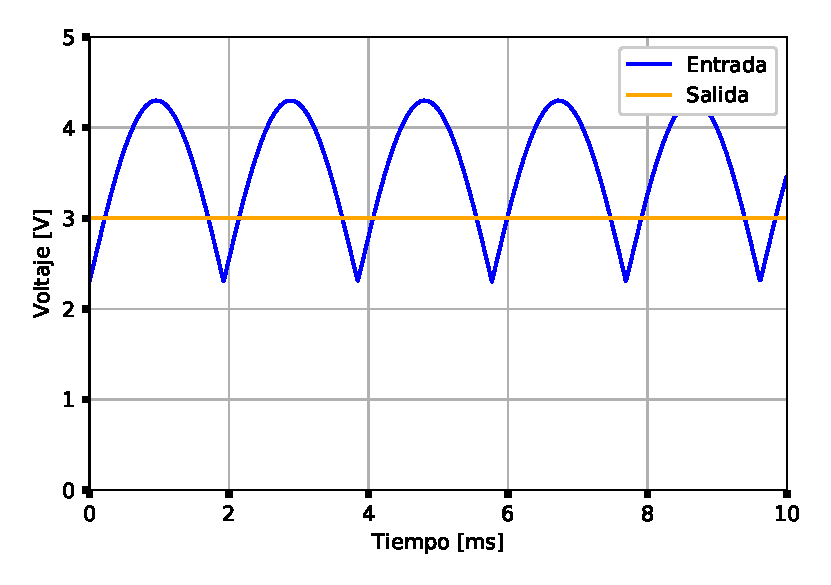
\includegraphics[width=.8\textwidth]{Figures/filtro_graf.eps}
\caption[Simulación del filtro pasabajas]{La señal de entrada corresponde a la señal que entrega la etapa rectificadora (azul), al aplicar el filtro capacitivo se obtiene una señal continua (amarilla) que es proporcional al campo eléctrico.}
\label{pbgraf}
\end{center}
\end{figure}

\subsection{Digitalización}
% README: ADC PSOC y sus caracterizticas
Uno de los objetivos de la estación es transmitir los datos utilizando protocolo I$^{2}$C, por lo que fue necesario digitalizar la señal de DC proporcional al campo eléctrico atmosférico que se obtuvo en la etapa del filtro pasabaja.

\begin{figure}[H]
 \centering
  \subfloat[]{
   \label{p1}
    \includegraphics[width=0.3\textwidth]{Figures/digitalizacion.eps}}
  \subfloat[]{
   \label{p2}
    \includegraphics[width=0.55\textwidth]{Figures/adc_config.PNG}}
 \caption[Módulo ADC SAR del PSOC 5LP]{(a) Digitalización de la señal de CC, con un ADC de tipo SAR, embebido en la tarjeta PSOC 5 LP . (b) Configuración del modulo ADC de la tarjeta PSOC 5LP.}
 \label{adc_muestreo}
\end{figure}
La digitalización de la señal, se hizo con un ADC delta-sigma de 20 bits el cual esta embebido en la tarjeta PSOC 5LP. En la Fig. \ref{adc_muestreo} se muestra el módulo del ADC y sus parámetros de configuración, los cuales se puede encontrar en las librerías del programa PSOC Creator en su versión 4.2. Para la configuración del módulo se seleccionó entrada tipo (Single ended) de 20 bits, frecuencia de muestreo de 183 SPS, rango de entrada de Vssa a Vdda, modo de conversión continuo, modo rail to rail del buffer y voltaje de referencia de Vdda/4.\\

\begin{figure}[h!]
\begin{center}
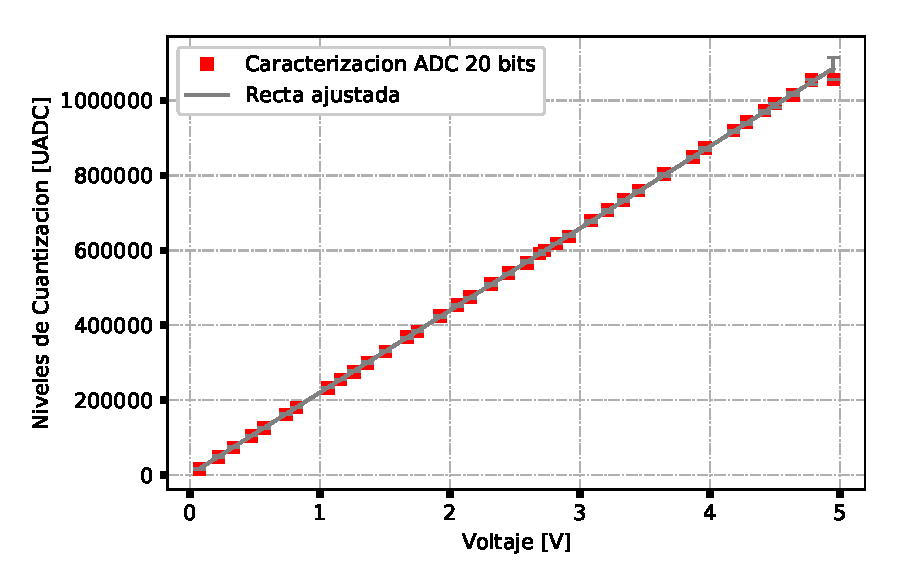
\includegraphics[width=0.8\textwidth]{Figures/ADC.eps}
\caption[Calibración del ADC SAR del PSOC 5LP]{Calibración del ADC tipo SAR embebido en la tarjeta PSOC 5LP, donde podemos observar que 1 UADC equivale a aproximadamente 4,5 $\mu$V}%CYPRESS   
\label{adc_curve}
\end{center}
\end{figure}
La caracterización del ADC se realizó aplicando un voltaje en su entrada y observando el valor de conversión medido. En la Fig. \ref{adc_curve} se muestra la gráfica de la calibración que se obtuvo, en donde podemos observar que 1 UADC equivale a aproximadamente 4,5 $\mu$V.


\subsection{Transmisión de datos}
% README: Transmisión i2c con el 
La transmisión se hizo con la tarjeta PSOC 5LP que cuenta con un módulo I$^{2}$C. En la Fig. \ref{transmision} se encuentra el módulo EZI2C y sus parámetros de configuración, se seleccionó una velocidad de transmisión de 100 kbps, una dirección esclava y pines conexión predeterminados. Para implementar el módulo se utilizó un código en lenguaje de programación C (ver Anexo \ref{adc_i2c}), el cual inicializa el módulo, define la dirección del módulo en 0x60 y finalmente transmite los valores que se le asignan al buffer donde se almacenan los datos medidos por el ADC.\\

\begin{figure}[h!]
 \centering
  \subfloat[]{
   \label{tra1}
    \includegraphics[width=0.35\textwidth]{Figures/transmicion.eps}}
  \subfloat[]{
   \label{tra2}
    \includegraphics[width=0.65\textwidth]{Figures/i2c_config.PNG}}
 \caption[Módulo I2C del PSOC 5LP]{(a) Transmisión de los valores en memoria mediante el módulo I$^{2}$C, embebido en la tarjeta PSOC 5 LP . (b) Configuración del módulo I$^{2}$C.}
 \label{transmision}
\end{figure}
En la Fig. \ref{i2c_pines} se encuentra los pines del PSOC 5LP utilizados por el sensor de campo eléctrico. Se definieron los pines P12[1] (sda) y P12[0] (scl) para la transmisión I$^{2}$C.

\begin{figure}[h!]
\begin{center}
\includegraphics[width=0.8\textwidth]{Figures/pines.png}
\caption{Pines utilizados por la tarjeta PSOC 5LP}
\label{i2c_pines}
\end{center}
\end{figure}
Se digitalizó una señal triangular utilizando el ADC tipo SAR y se transmitió vía I$^{2}$C. En los resultados se encontró que los datos recibidos tenían errores. Estos errores se debían a que mientras que el ADC guarda el valor digitalizado en memoria, el I$^{2}$C intenta leerlo, causando un error de lectura, por lo que se puso un tiempo de espera en la transmisión de 100 ms, para dar tiempo al ADC de registrar los valores medidos. 

\section{Calibración}
% README: Generador de campo eléctrico controlado y calibración hecha.
\subsection{Caracterización del generador de campo }
La calibración del sensor de campo eléctrico lento, se realizó utilizando un generador de campo controlado. Dicho generador está compuesto por un capacitor cuadrado de placas paralelas de 20 cm x 20 cm de área y 10 cm de separación, cuya capacitancia es de 3.54 $p$F. En la Fig. \ref{cap} se observa un esquema del montaje, se utilizaron tubos de PBC para separar y aislar eléctricamente los platos de baquela, la cual posee un recubrimiento de cobre de 35 $\mu$m.\\

\begin{figure}[h!]
\begin{center}
\includegraphics[width=0.8\textwidth]{Figures/calibracion_esquema.eps}
\caption[Esquema de los platos del generador de campo eléctrico controlado]{Fuente de campo eléctrico controlado que genera de 0 V/m a 20 kV/m, por medio de una fuente programable de alto voltaje DC/DC EMCO C20.}
\label{cap}
\end{center}
\end{figure}
Para el proceso de calibración se tuvo en cuenta la metodología propuesta por Cui et. al. \cite{cui2017model}, que establece el proceso a seguir para la calibración del sensor de campo eléctrico tipo molino, utilizando un capacitor de placas paralelas que genera un campo eléctrico controlado. El campo producido por un capacitor de placas paralelas se puede describir por la expresión de la Eq. \ref{campo}.
\begin{equation}
     E = \frac{V}{d}
     \label{campo}
\end{equation}
Donde E es el campo eléctrico, V es el voltaje entre las placas y d la distancia de separación. Se estableció una distancia fija de 10 cm, con el fin de controlar el valor del campo inducido entre las placas, regulando el voltaje aplicado. En este caso se utilizó una fuente DC/DC EMCO C20 programable de alta precisión. El control del generador de campo se hace mediante una señal de 0 a 5 V (Vctrl), lo que produce en la fuente DC/DC un voltaje de salida de 0 a 2 kV y en el capacitor de placas paralelas campos eléctricos entre 0 y 20 kV/m.\\

\begin{figure}[h!]
\begin{center}
\includegraphics[width=0.89\textwidth]{Figures/Esq_Ectrl.eps}
\caption[Esquema general del generador de campo eléctrico controlado]{Esquema general del generador de campo eléctrico, se utiliza una interfaz en Python programada en un Raspberry Pi para configurar los valores de voltaje de control vía ethernet desde un servidor, la fuente EMCO C20 genera voltajes entre 0 y 2 kV lo que establece un campo eléctrico entre la placas en un rango de 0 a 20 kV/m.}
\label{esq_ectrl}
\end{center}
\end{figure}
En la Fig. \ref{esq_ectrl} se muestra el esquema del banco de prueba implementado para el proceso de calibración. Mediante una interfaz creada en Python se configura el campo eléctrico aplicado a las placas del capacitor. Para ello se utiliza el DAC MCP4725 de 12 bits obteniéndose una resolución de $\sim$5 V/m. El DAC es controlado por una interfaz I$^{2}$C desde una Raspberry Pi conectada vía ethernet a un servidor.\\

\begin{figure}[H]
\begin{center}
\includegraphics[width=0.80\textwidth]{Figures/Fuente_E.eps}
\caption{Calibración del generador de campo eléctrico programable.}
\label{cal_fuente}
\end{center}
\end{figure}
Antes de calibrar el sensor de campo lento es necesario caracterizar el generador de campo eléctrico, para ello se aplicaron voltajes en un rango de 0 a 5 V con pasos de 0.1 V desde una interfaz en Python. Los resultado obtenidos se muestra en la Fig. \ref{cal_fuente}, donde se observa que la curva obtenida se ajusta a una recta que varia 4.095 V/m por cada mV en el Vctrl.

\subsection{Calibración del sensor}
referenciar la norma de calibración

IEEE Guide for the Measurement of DC Electric-Field Strength and Ion Related Quantities

y este artículo

Model, Design, and Testing of Field Mill Sensors for Measuring Electric Fields Under High-Voltage Direct-Current Power Lines, Yong Cui, 2018

Para la calibración del sensor de campo eléctrico lento, se ubicó el sensor entre las placas del capacitor tal como se muestra en la Fig. \ref{cap}, a continuación se generaron campos entre 0 y 20 kV/m con pasos de $\sim$400 V/m. Los resultados obtenido se muestran en la Fig. \ref{emill_graf}, donde se observa que la curva obtenida se ajusta a una recta que varía a razón de 90.6 mV por cada kV/m aplicado.

\begin{figure}[h!]
\begin{center}
\includegraphics[width=.85\textwidth]{Figures/Emill_Completo.eps}
\caption{Calibración del sensor de campo eléctrico, bajo condiciones ideales.}
\label{emill_graf}
\end{center}
\end{figure}


\section{Primeras mediciones}
% REAME: Gráficas de las mediciones hechas por la estación, descripción del comportamiento del campo eléctrico.
El prototipo de sensor de campo eléctrico, se instaló en una plataforma elevada a 3 m del suelo, con una estructura en tubos de PVC, ya que estos se construyen para resistir la intemperie, la estructura es modular, tal como se observa en la Fig. \ref{estructura}. El sensor se ubica de forma vertical en el extremo de la estructura, por lo que los platos quedan invertidos, esto se considera a la hora de interpretar, los datos registrados.\\

\begin{figure}[H]
 \centering
  \subfloat[]{
   \label{real_estr}
    \includegraphics[width=0.5\textwidth]{Figures/estructura.jpeg}}
  \subfloat[]{
   \label{esq_estr}
    \includegraphics[width=0.5\textwidth]{Figures/estructura.eps}}
 \caption[Estructura mecánica del sensor de campo lento]{(a) Estructura mecánica hecha en PVC, que soporta al sensor de campo eléctrico lento. (b) Esquema de la estructura mecánica del sensor de campo eléctrico lento, con sus respectivas dimensiones.}
 \label{estructura}
\end{figure}
Las primeras mediciones del sensor captaron se realizaron los días 08, 09 y 10 de Noviembre del año 2019 en la ciudad de Bucaramanga, Santander en el observatorio del grupo Halley de la Universidad Industrial de Santander. En la Fig. \ref{med} se puede observar los datos del campo eléctrico registrado. Xu B. et. al. encontraron que el campo eléctrico diurno en condiciones normales (fairweather), varía entre 50 y 220 V/m \cite{xu2013periodic}, lo cual concuerda con las mediciones realizadas por el prototipo.\\

\begin{figure}[h!]
\begin{center}
\includegraphics[width=0.8\textwidth]{Figures/mediciones.eps}
\caption[Registro de las primeras mediciones realizadas con el sensor]{Registro de campo eléctrico atmosférico hechas con el primer prototipo de sensor tipo molino los días 08, 09 y 10 de Noviembre del año 2019, donde se resalta el campo eléctrico en un día con condiciones normales, campo eléctrico nocturno y los eventos registrados para un día de tormenta.}
\label{med}
\end{center}
\end{figure}
El campo eléctrico nocturno durante los días de registro mostraba un aumento debido a la acumulación de nubes sobre el sensor por la disminución de temperatura ambiente. En una tormenta eléctrica el campo eléctrico atmosférico varía debido a descargas atmosféricas y acumulación de carga en las nubes \cite{xu2013periodic}. En la Fig. \ref{tormenta} se observa el comportamiento del campo eléctrico atmosférico el día 09 de Noviembre del año 2019 entre las 3 am y 5 am en la ciudad de Bucaramanga, en donde se presentaron precipitaciones y tormentas eléctricas. 

\begin{figure}[h!]
\begin{center}
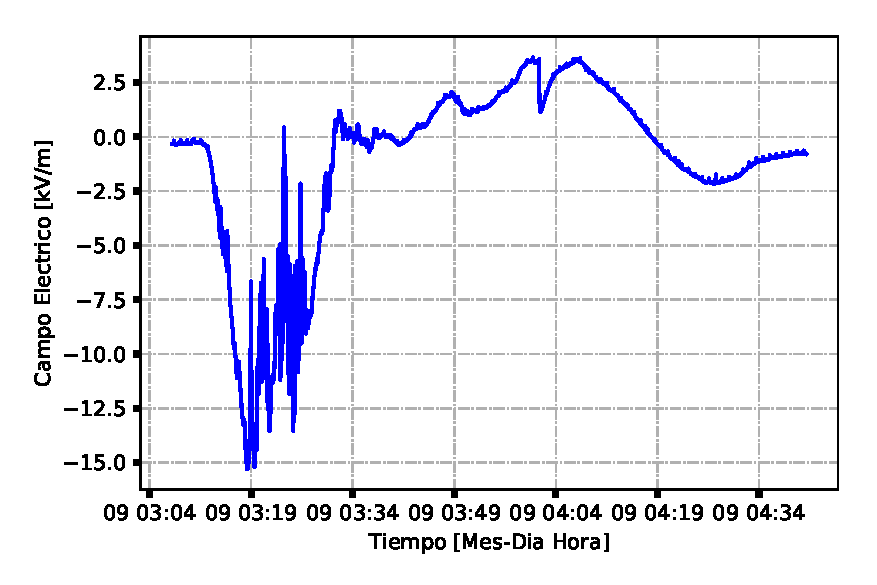
\includegraphics[width=0.8\textwidth]{Figures/tormenta.eps}
\caption[Registro de las primeras mediciones de tormentas eléctricas]{Registro de campo eléctrico atmosférico hechas con el primer prototipo de sensor tipo molino el día 09 de Noviembre del año 2019 entre las 3 am y 5 am en la ciudad de Bucaramanga, en donde ocurrieron algunas tormentas eléctricas.}
\label{tormenta}
\end{center}
\end{figure}

